\documentclass[UTF8,oneside]{ctexbook}
\usepackage{graphicx} % 插图
\graphicspath{{img/}}
\usepackage{pdfpages} % 首页大图
% 简单的 代码高亮
\usepackage{listings}
\usepackage{xcolor}
\lstset{
    basicstyle=\ttfamily\small, % 小字号
    columns=fixed,       
    numbers=left, % 在左侧显示行号
    frame=none, % 不显示背景边框
    backgroundcolor=\color[RGB]{245,245,244},  % 设定背景颜色
    keywordstyle=\color[RGB]{40,40,255}\bfseries, % 设定关键字颜色
    numberstyle=\footnotesize\color{darkgray}, % 设定行号格式
    commentstyle=\color[RGB]{0,96,96}, % 设置代码注释的格式
    stringstyle=\slshape\color[RGB]{128,0,0}, % 设置字符串格式
    showstringspaces=false, % 不显示字符串中的空格
}
% \usepackage{hyperref} % URL
% \usepackage{makeidx}
% \makeindex
% \bibliographystyle{...}


%% 文档开始 ===================================================
\begin{document}

%% 首页
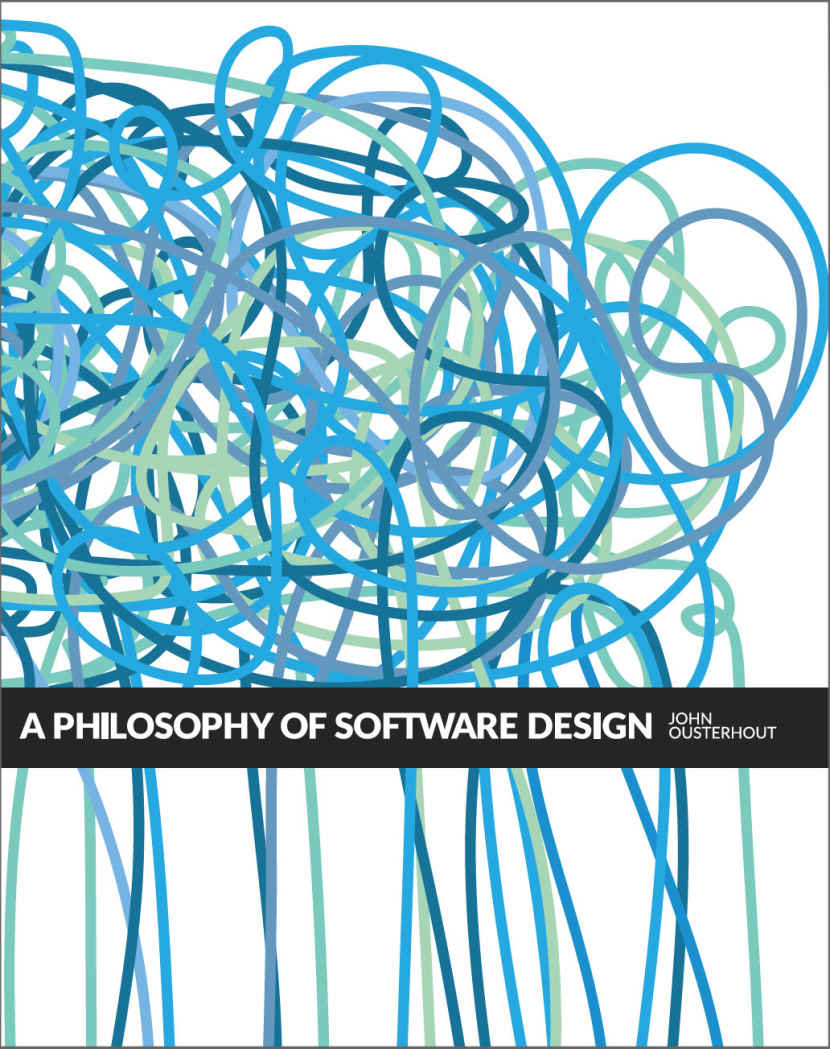
\includepdf[fitpaper=true]{img/cover.jpg}

%% 新开一页
\frontmatter
\title{《软件设计的哲学》中文版}
\author{ John Ousterhout }
\date{\today}
\maketitle % 标题页
% 简介
斯坦福教授、Tcl 语言发明者 John Ousterhout 的著作《A Philosophy of Software Design》,自出版以来,好评如潮。按照 IT 图书出版的惯例,如果冠名为“实践”,书中内容关注的是某项技术的细节和技巧;冠名为“艺术”,内容可能是记录一件优秀作品的设计过程和经验;而冠名为“哲学”,则是一些通用的原则和方法论,这些原则方法论串起来,能够形成一个体系。正如”知行合一”、“世界是由原子构成的”、“我思故我在”,这些耳熟能详的句子能够一定程度上代表背后的人物和思想。用一句话概括《A Philosophy of Software Design》,软件设计的核心在于降低复杂性。

% 前言
\input{chaps/preface.tex}
% 目录
\tableofcontents
\mainmatter

%% 正文部分 ---------------------
%% 1~21 章
\input{chaps/ch1.tex}
\input{chaps/ch2.tex}
\input{chaps/ch3.tex}
\input{chaps/ch4.tex}
\input{chaps/ch5.tex}
\input{chaps/ch6.tex}
\input{chaps/ch7.tex}
\input{chaps/ch8.tex}
\input{chaps/ch9.tex}
\input{chaps/ch10.tex}
\input{chaps/ch12.tex}
\input{chaps/ch13.tex}
\input{chaps/ch14.tex}
\input{chaps/ch15.tex}
\input{chaps/ch16.tex}
\input{chaps/ch17.tex}
\input{chaps/ch18.tex}
\input{chaps/ch19.tex}
\input{chaps/ch20.tex}
\input{chaps/ch21.tex}
%% 总结
\input{chaps/summary.tex}
%% 正文部分结束 -------------------

%% 后记
% \backmatter
% \bibliography{...} % 参考文献
% \printindex

\end{document} %% 文档结束 ====================================